\documentclass[prd,aps,10pt,nofootinbib,twocolumn,superscriptaddress,preprintnumbers,balancelastpage,longbibliography]{revtex4-1}

\usepackage{amsmath,amssymb}	
\usepackage{mathtools}
\usepackage{fontawesome}
\usepackage[dvipsnames]{xcolor}
\usepackage{hyperref}
\usepackage{xspace}
\usepackage{fancyhdr}
\usepackage{braket}
\usepackage{graphicx}
\usepackage{siunitx}
\usepackage{blindtext}
\usepackage{nicefrac}
\usepackage{lipsum}

\usepackage{afterpage}
\newcolumntype{L}[1]{>{\raggedright\let\newline\\\arraybackslash\hspace{0pt}}m{#1}}
\newcolumntype{C}[1]{>{\centering\let\newline\\\arraybackslash\hspace{0pt}}m{#1}}
\newcolumntype{R}[1]{>{\raggedleft\let\newline\\\arraybackslash\hspace{0pt}}m{#1}}
\usepackage{longtable}
\setlength{\LTcapwidth}{\textwidth}

\newcommand{\nbicon}{{\color{linkcolor}\faFileCodeO}\xspace}
\newcommand{\nblink}[1]{\href{https://github.com/smsharma/dark-photons-perturbations/blob/apr-2020/notebooks/#1.ipynb}{\nbicon}}
\newcommand{\githubmaster}{\href{https://github.com/smsharma/dark-photons-perturbations/}{\faGithub}\xspace}

\newcommand{\dd}{\mathrm{d}}
\newcommand{\mAp}{m_{A^\prime}}
\newcommand{\vect}[1]{\boldsymbol{\mathbf{#1}}}

\definecolor{deepgreen}{rgb}{0.2,0.8,0.2}
\newcommand{\SM}[1]{{\bf \color{deepgreen}{[SM: #1]}}}

\colorlet{linkcolor}{BrickRed}



\hypersetup{colorlinks=true,
linkcolor=linkcolor,
citecolor=linkcolor,
urlcolor=linkcolor,
,linktocpage=true
,pdfproducer=medialab}

\DeclareSIUnit \h {\ensuremath{\mathit{h}}}
\DeclareSIUnit\electronvolt{e\kern-.05em V}
\DeclareSIUnit\parsec{pc}

\begin{document}

\title{A neural simulation-based inference approach for characterizing \\ the Galactic Center $\gamma$-ray excess}
 
\author{Siddharth Mishra-Sharma}
\email{sm8383@nyu.edu}
\thanks{ORCID: \href{https://orcid.org/0000-0001-9088-7845}{0000-0001-9088-7845}}
\affiliation{Center for Cosmology and Particle Physics, Department of Physics, New York University, New York, NY 10003, USA}

\author{Kyle Cranmer}
\email{kyle.cranmer@nyu.edu}
\thanks{ORCID: \href{https://orcid.org/0000-0002-5769-7094}{0000-0002-5769-7094}}
\affiliation{Center for Cosmology and Particle Physics, Department of Physics, New York University, New York, NY 10003, USA}
\affiliation{Center for Data Science, New York University, 60 Fifth Ave, New York, NY 10011, USA}

\date{\today}

\begin{abstract}
The nature of the \Fermi $\gamma$-ray Galactic Center Excess (GCE) has remained a persistent mystery for over a decade. Although the excess is broadly compatible with emission expected from annihilating dark matter, an explanation in terms of a population of unresolved point sources remains viable. The effort to uncover its origin is hampered in particular by the mischaracterization of the diffuse emission of Galactic origin, which can lead to spurious residuals that make it difficult to robustly differentiate smooth emission, as expected of dark matter origin, from more clumpy emission sources from relatively bright, unresolved point sources. We use neural simulation-based inference methods, in particular conditional density estimation, in order to extract more information from $\gamma$-ray maps of the Galactic Center with the aim of characterizing the contribution of unresolved point sources to the GCE.
\end{abstract}

\maketitle

\section{Introduction}
\label{sec:intro}

Dark matter (DM) represents one of the major unsolved problems in particle physics and cosmology today. The traditional Weakly-Interacting Dark Matter (WIMP) paradigm envisions production of dark matter in the early Universe through freeze-out of dark matter particles weakly coupled to the Standard Model (SM). In this scenario, one of the most promising methods of detecting a dark matter signal would be through an excess of $\gamma$-ray photons from DM-rich regions of the sky, produced through the cascade of SM particles produced as a result of DM annihilation. 

The \Fermi $\gamma$-ray Galactic Center Excess (GCE), first identified over a decade ago using data from the \Fermi Large Area Telescope (LAT), is an excess of photons in the Galactic Center with properties---such as energy spectrum and spatial morphology---roughly compatible with that expected due to annihilation DM. The nature of the GCE remains contentious---although it's properties are similar to that expected from DM annihilation, competing explanations in terms of a population of unresolved astrophysical point sources (PSs) remain viable. Although analyses based on the statistics of photon counts in the Galactic Center have shown the data to prefer a point source origin of the excess, recent analyses have pointed out the potential of unknown systematics in the data---such as the morphology of the diffuse foreground emission---to bias the conclusions of these results. Furthermore, analyses of the spatial morphology of the excess have shown it to be more compatible with that tracing a stellar bulge distribution in the Galactic Center.

Novel analysis techniques that can extract more information from the high-dimensional photon count maps could do a better job of ``hedging'' against unknown systematics in the data compared to traditional analyses based on summary statistics like the 1-point PDF. Machine learning methods in particular have demonstrated promise for general analyses of $\gamma$-ray data and in particular focusing on understanding the nature of the GCE. In this paper, we leverage recent developments in the field of simulation-based inference (SBI) in order to weigh in on the nature of the GCE.

This paper is organized as follows. In Sec.~\ref{sec:analysis} we describe the various components of our analysis method based on simulation-based inference. In Sec.~\ref{sec:simulations} we describe our simulation pipeline and verify our analysis on simulated data. Section~\ref{sec:data} presents results on \Fermi $\gamma$-ray data. In Sec.~\ref{sec:mismodeling} we explore the susceptibility of the analysis to mismodeling of the background and signal templates, and present systematic variations on our analysis in Sec.~\ref{sec:systematics}. We conclude in Sec.~\ref{sec:conclusion}.

\section{Methodology}
\label{sec:analysis}

We begin by describing our analysis methodology, going over, in turn the general principles behind simulation-based inference, posterior estimation using normalizing flows, and learning representative summary statistics from high-dimensional $\gamma$-ray maps with neural networks.

\subsection{Simulation-based inference}

Of central interest in parameter estimation is often the probability distribution of a set of parameters of interest $\theta$ given some data $x$---the posterior distribution $p(\theta\mid x)$. Bayes' theorem can be used to obtain the posterior as $p(\theta\mid x) = p(\theta)\, p(x\mid\theta) / \mathcal Z$, where $p(x\mid\theta)$ is the likelihood and $\mathcal Z$ is the Bayesian evidence. In practice, parameters other than $\theta$---latent variables $z$---are often involved in the data-generation process, and computing the likelihood involves marginalizing over the latent space, $p(x\mid\theta) = \int \dd z\,p(x\mid\theta, z)$. In typical problems of interest, the high dimensionality of the latent space often means that this integral is intractable, necessitating simplifications in statistical treatment as well as theoretical modeling. 

% $\theta \sim p(\theta)$, $x\sim p(x\mid\theta, z)$, $z\sim p(z\mid\theta)$.

Simulation-based inference (SBI) refers to a class of methods for performing inference when the data-generating process does not have a tractable likelihood. In this setting, a model is defined through a simulator as a probabilistic program, often knows as a forward model. Samples $x$ from the simulator then implicitly define a likelihood, $x\sim p(x\mid\theta)$. In the simplest realizations of SBI, samples $x'$ generated from a given prior proposal distribution $p(\theta$) can be compared to a given dataset of interest $x$, with the approximate posterior defined by samples that most closely approximate $x$. Such methods---usually grouped under the umbrella term Approximate Bayesian Computation (ABC)---are not uncommon in astrophysics and cosmology. Nevertheless, they suffer from several downsides. The curse of dimensionality usually necessitates reduction of data to representative lower-dimensional summary statistics $s(x)$, resulting in loss of information. A notion and measure of distance between summaries from the implicit model and those derived from the dataset of interest is necessary, leading to inexact inference. Additionally, the ABC analysis must be performed anew for each new target dataset.

Recently, methods leveraging advancements in machine learning and probabilistic programming have been developed in order to address these issues, enabling new ways of performing inference on complex models defined through simulations. See Ref. for a review of recent developments.

\subsection{Conditional density estimation with normalizing flows}

In this paper, we approximate the joint posterior $p(\theta\mid x)$ through a parameterized distribution $\hat p_\phi(\theta\mid s)$ conditioned on summaries $s=s(x)$ from the samples $x$. This class of simulation-based inference techniques, known as conditional neural density estimation, directly models the posterior distribution given a set of samples drawn from simulator according to some prior proposal distribution $p(\theta)$.

We employ normalizing flows, which provide a general way of constructing flexible probability distributions, for posterior estimation. Specifically, we use Masked Autoregressive Flows (MAFs).

\subsection{Learning summary statistics with neural networks}

The curse of dimensionality makes it computationally prohibitive to condition the density estimation task on the the raw dataset $x$ \emph{i.e.}, the $\gamma$-ray pixel counts map in the region of interest (ROI). Instead, we use a neural network to learn lower-dimensional summary features from the map, $s = s_\varphi(x)$. The \emph{DeepSphere} architecture, with a configuration similar to that introduced and employed in Ref., is used here and summarized briefly here. For more details on the summary extractor network, see Ref.

\subsection{}

% based on Chebyshev spectral graph convolutions is used.

\section{Test on simulated data}
\label{sec:simulations}

%
\begin{figure*}
    \centering
    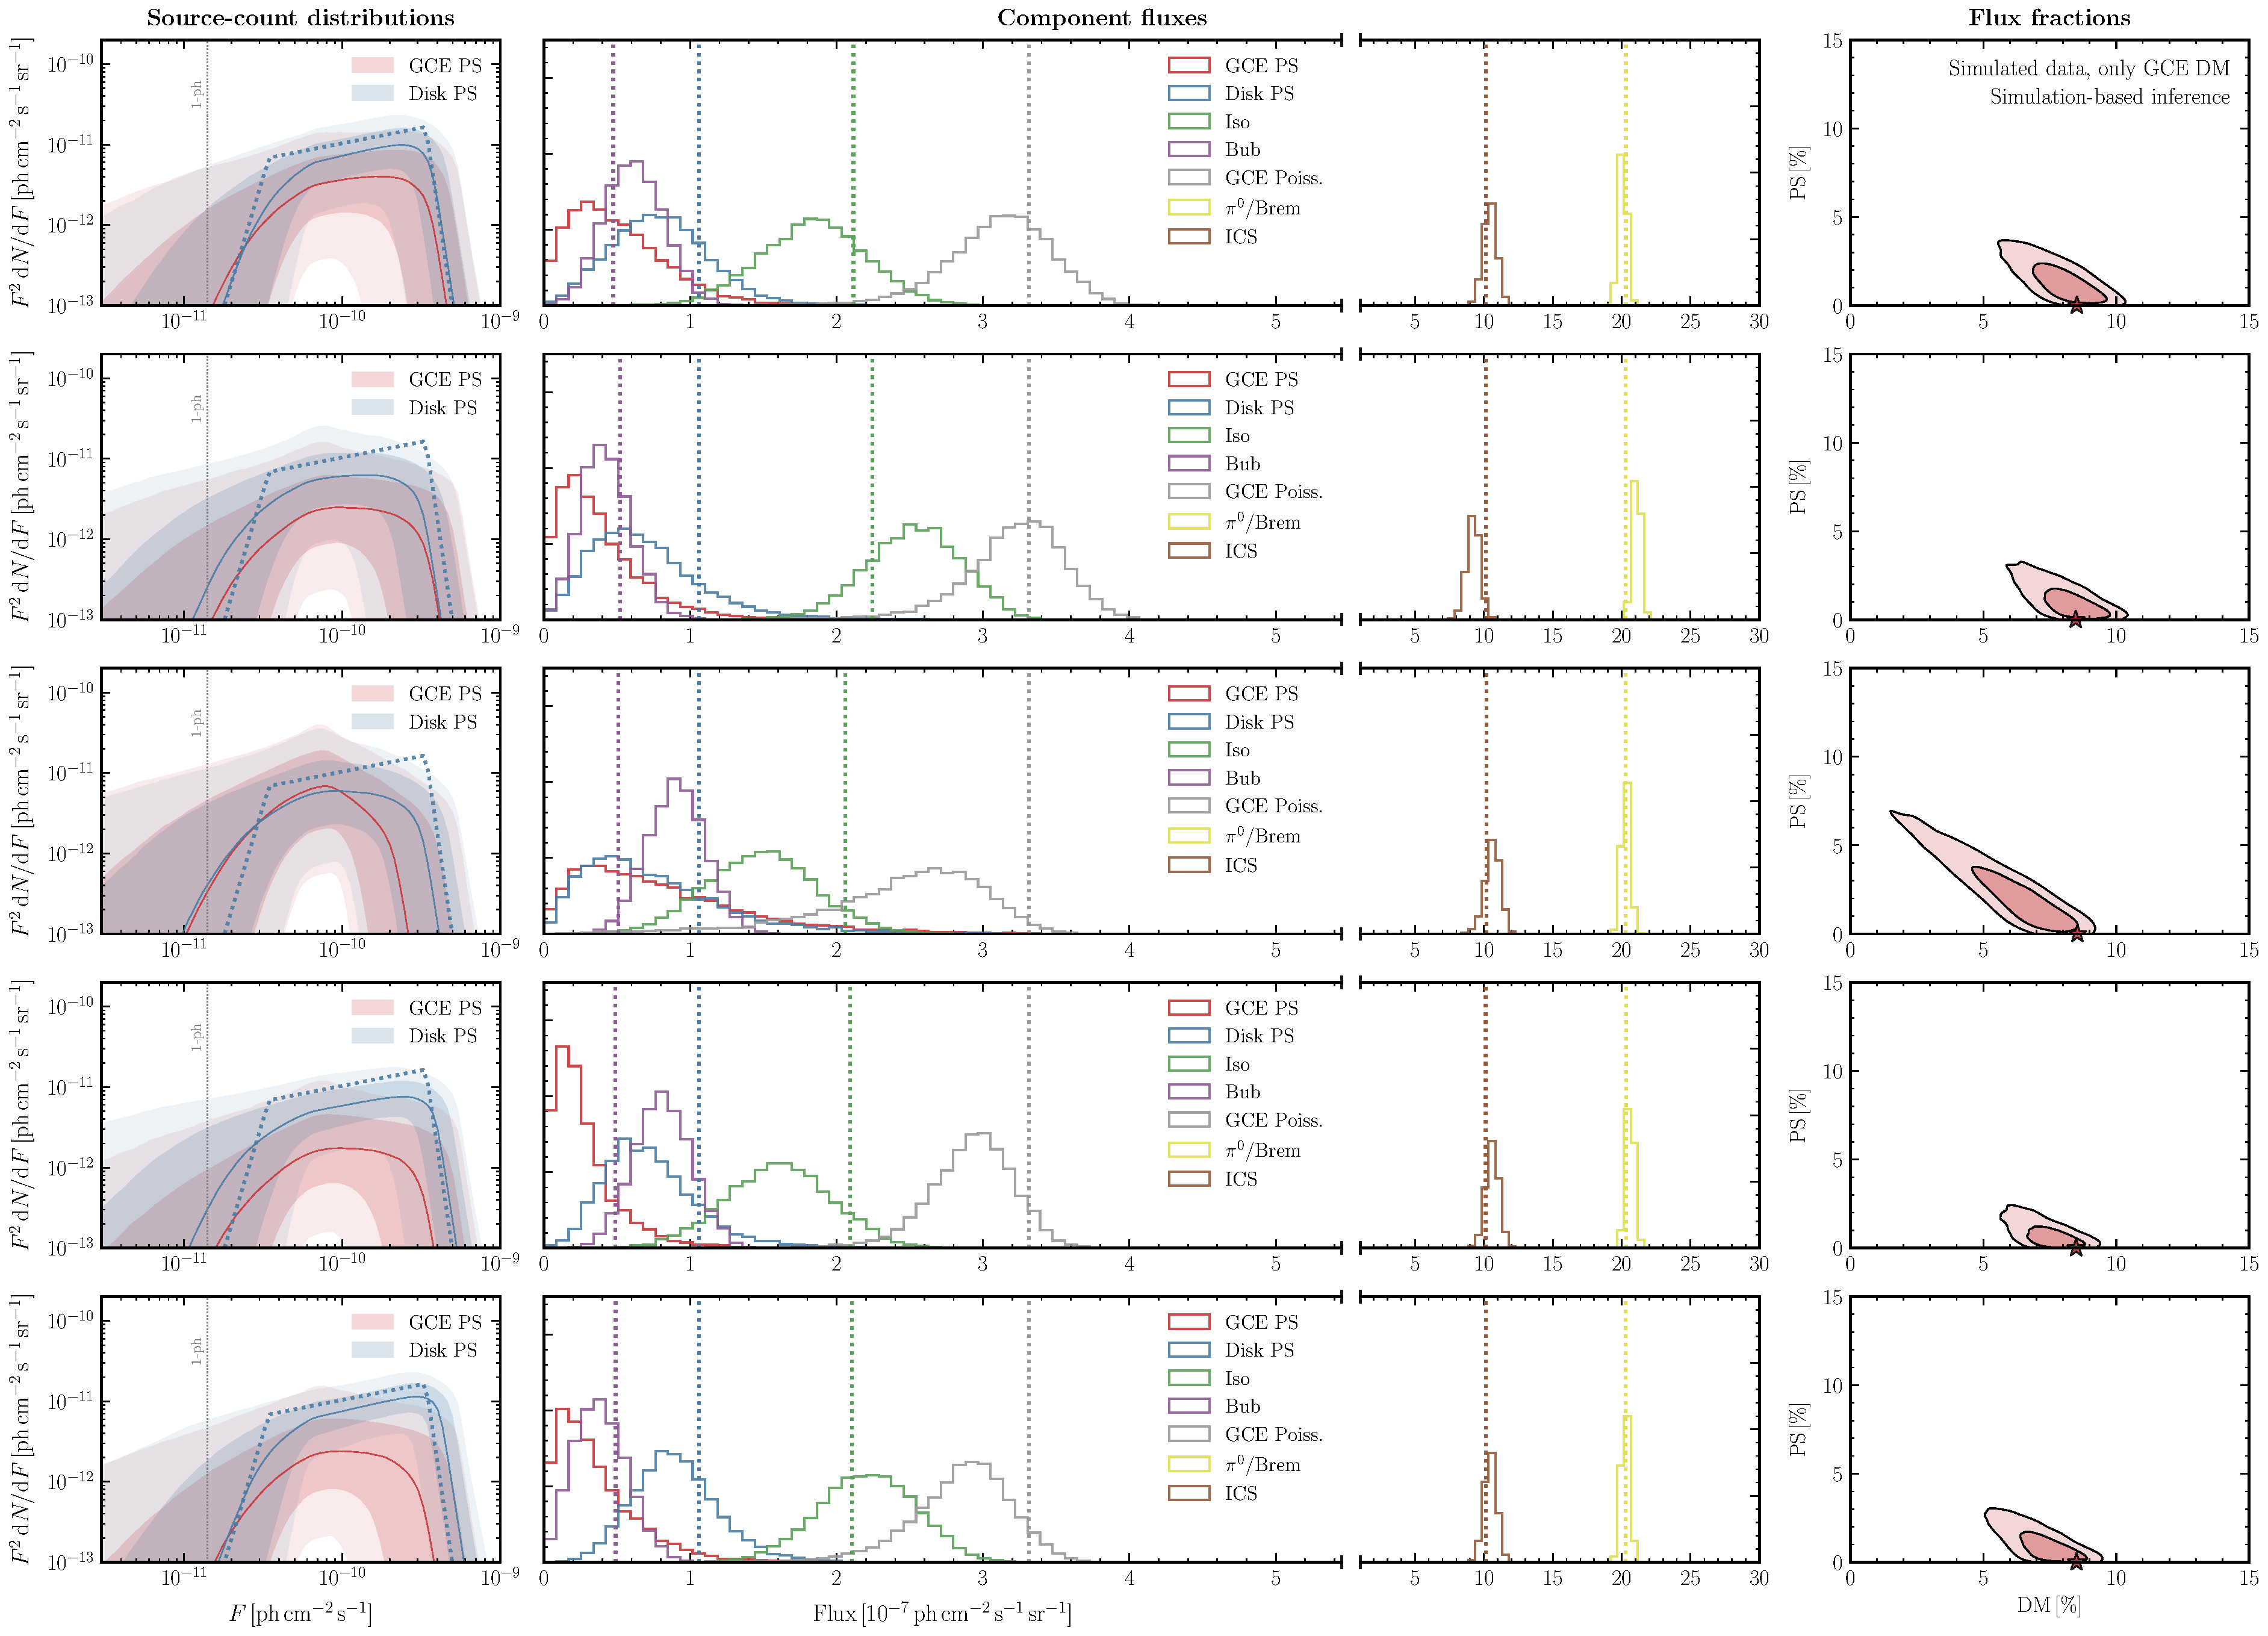
\includegraphics[width=0.95\textwidth]{plots/sim_sbi_dm.pdf}
    \caption{Results on simulated data where the GCE consists of purely PS-like emission.}
    \label{fig:sim_sbi_dm}
\end{figure*}
%

%
\begin{figure*}
    \centering
    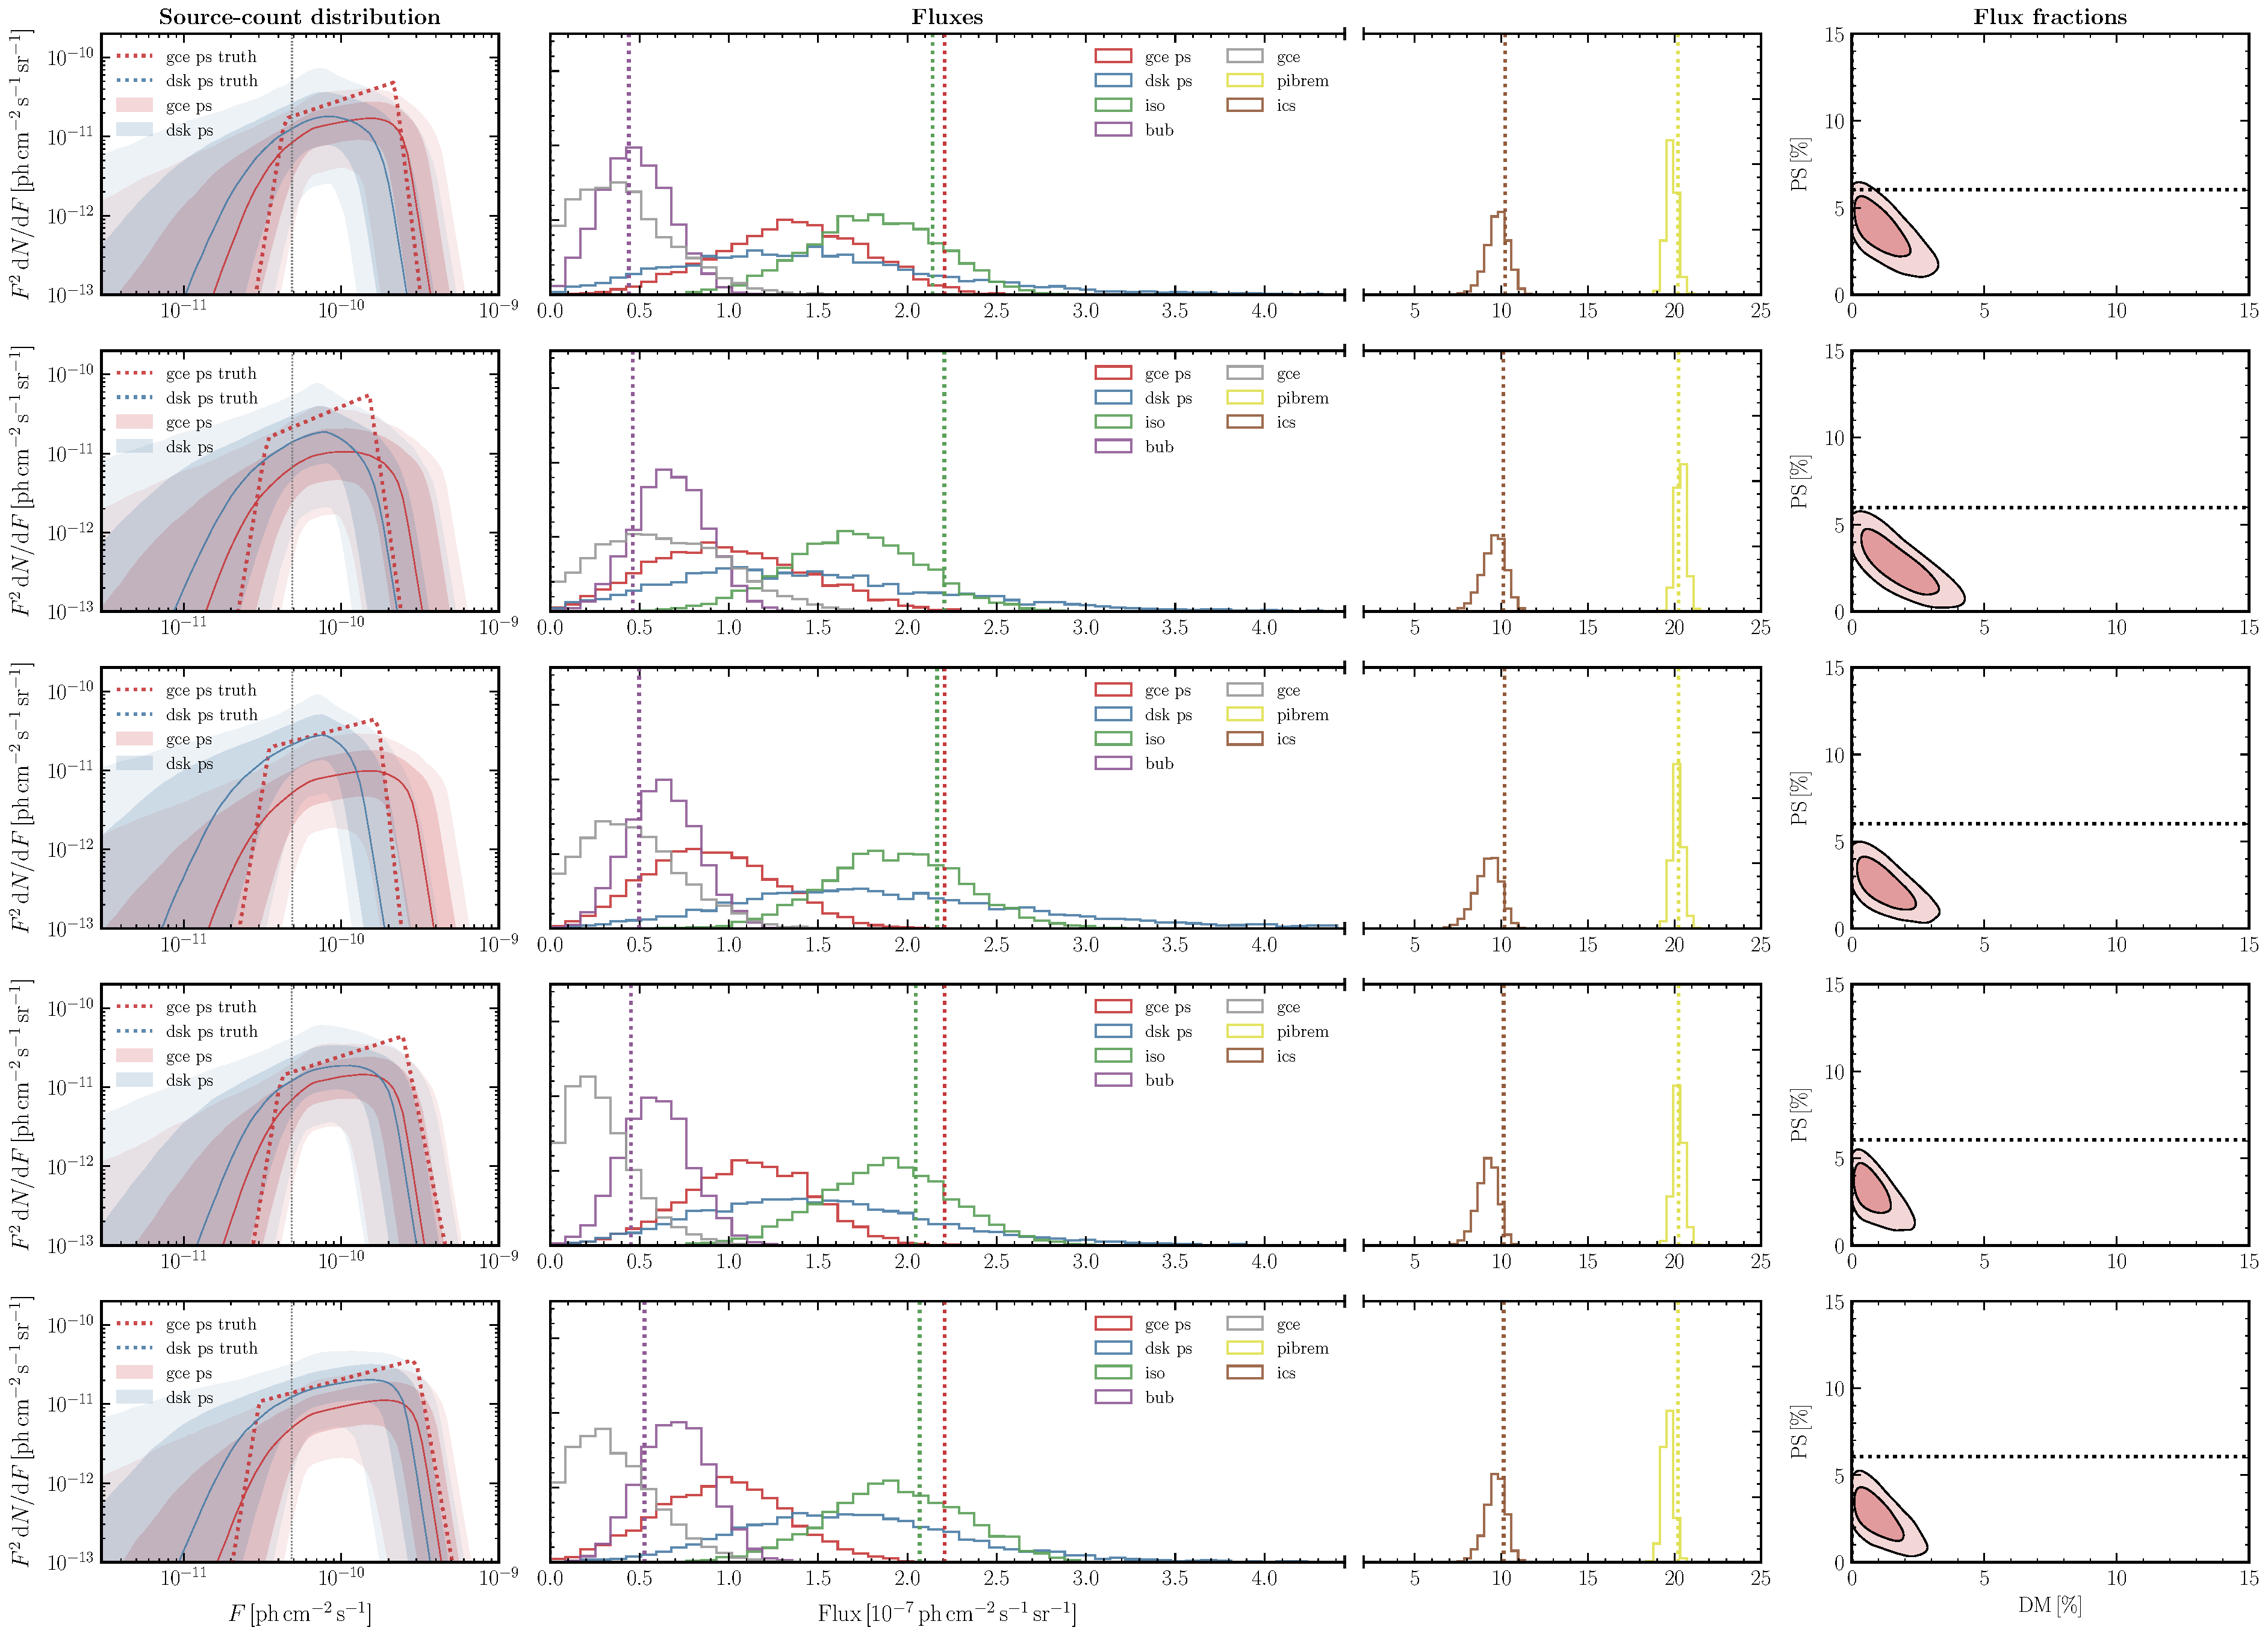
\includegraphics[width=0.95\textwidth]{plots/sim_sbi_ps.pdf}
    \caption{Results on simulated data where the GCE consists of purely DM-like emission.}
    \label{fig:sim_sbi_ps}
\end{figure*}
%

\section{Results on \emph{Fermi} data}
\label{sec:data}

%
\begin{figure*}
    \centering
    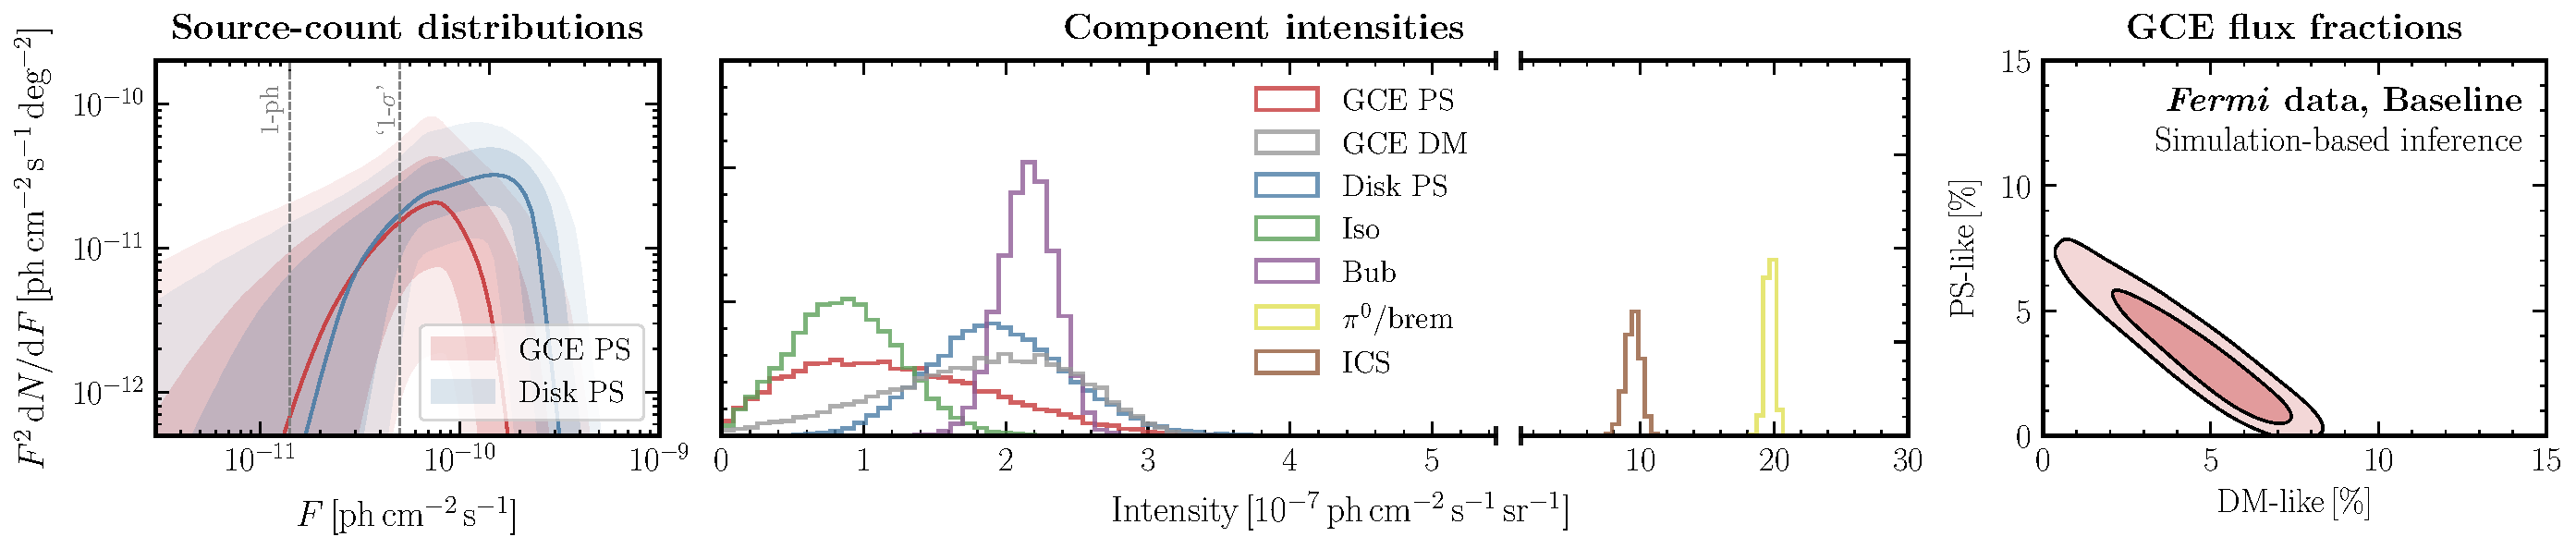
\includegraphics[width=0.95\textwidth]{plots/data_fid_sbi.pdf}
    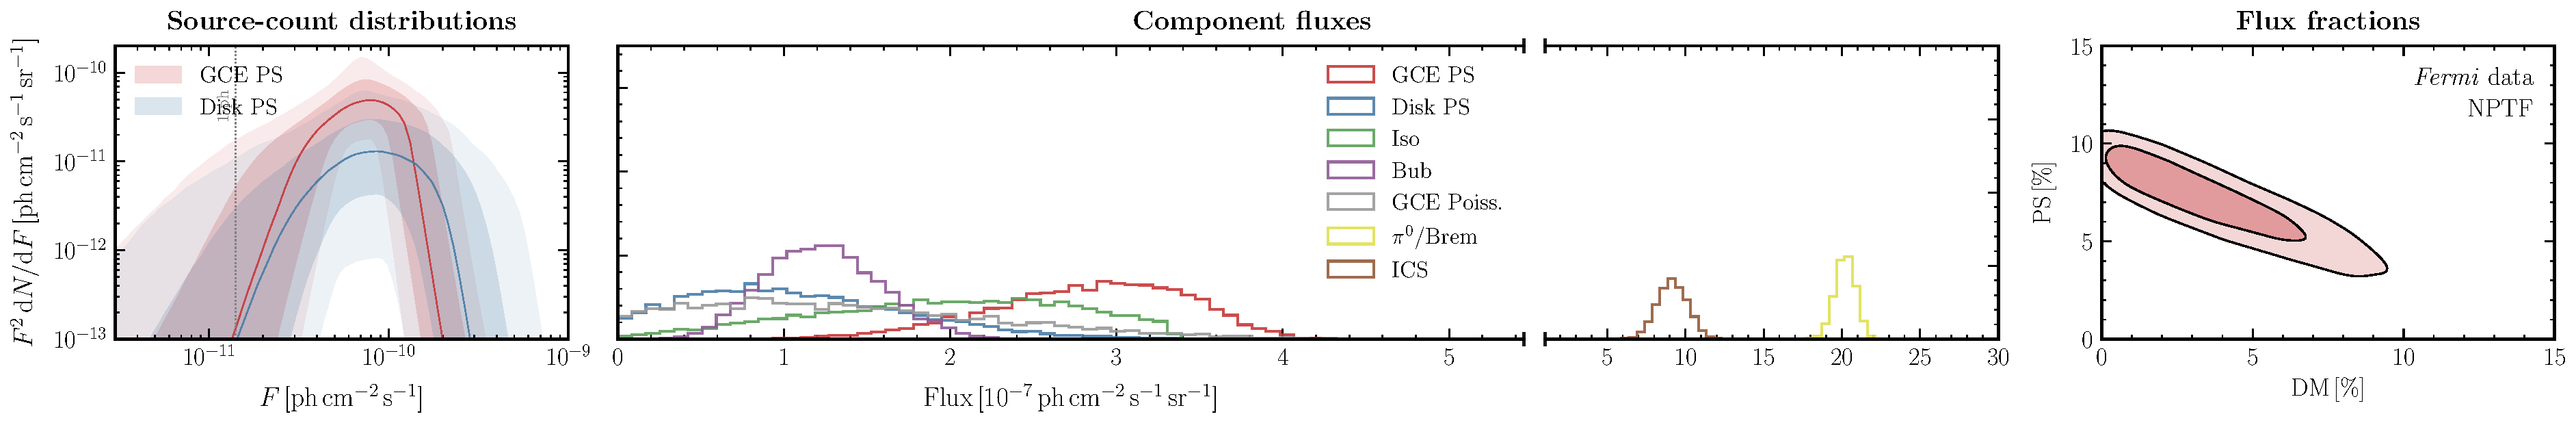
\includegraphics[width=0.95\textwidth]{plots/data_fid_nptf.pdf}
    \caption{Fiducial results on data.}
    \label{fig:fid_data}
\end{figure*}
%

\subsection{Signal injection test}
\label{sec:sig-injection}

%
\begin{figure*}
    \centering
    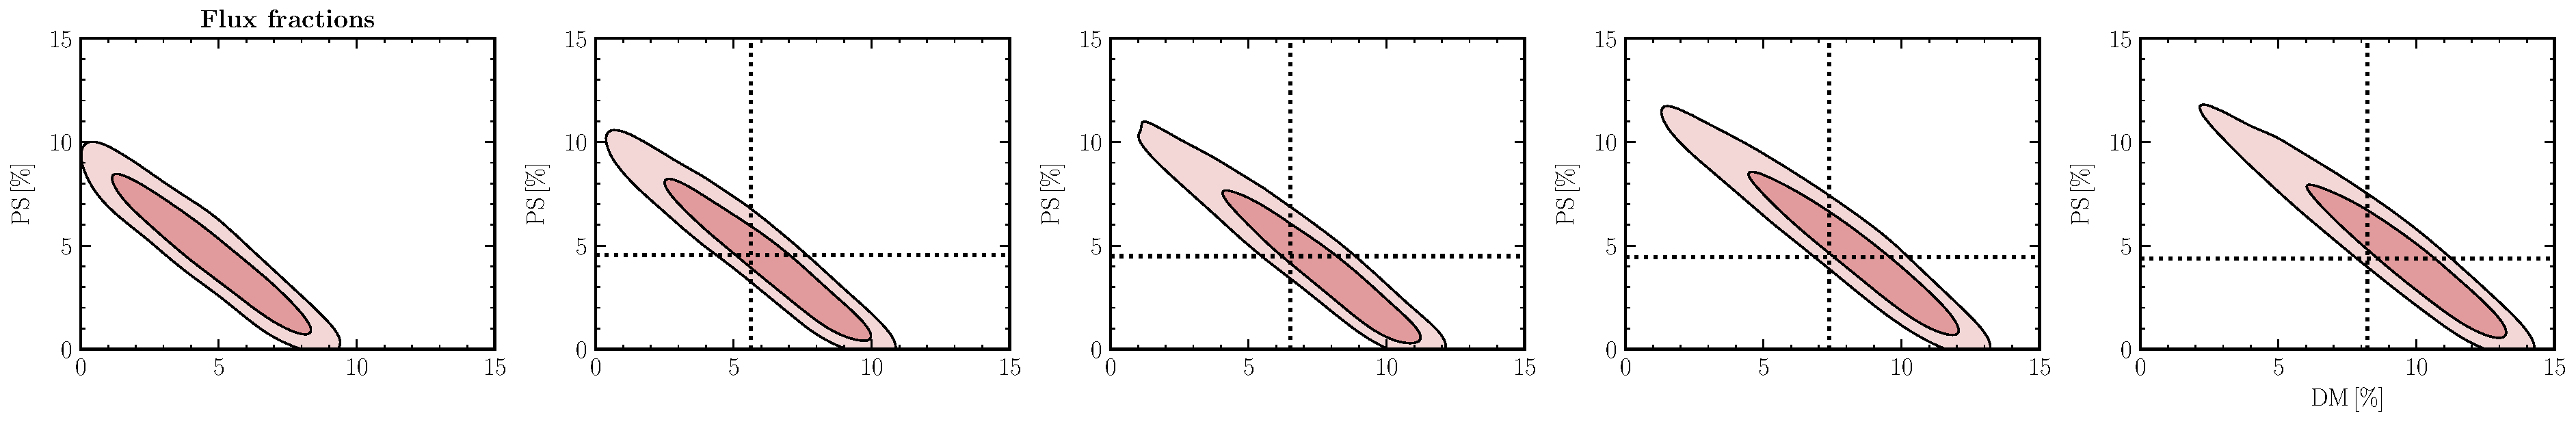
\includegraphics[width=0.95\textwidth]{plots/data_sig_inj.pdf}
    \caption{Signal injection on data.}
    \label{fig:sig_inj_data}
\end{figure*}
%

\section{Susceptibility to mismodeling}
\label{sec:mismodeling}

\subsection{Foreground mismodeling}
\label{sec:fg-mismodeling}

\subsection{Signal mismodeling}
\label{sec:sig-mismodeling}

\section{Systematic variations on analysis}
\label{sec:systematics}

\section{Conclusions}
\label{sec:conclusion}

\vspace{.3cm}
%%%%%%%%%%%%%%%

\begin{acknowledgments}

We thank\ldots for helpful conversations.  
KC is partially supported by NSF awards ACI-1450310, OAC-1836650, and OAC-1841471, the NSF grant PHY-1505463, and the Moore-Sloan Data Science Environment at NYU. 
SM is supported by the NSF CAREER grant PHY-1554858, NSF grants PHY-1620727 and PHY-1915409, and the Simons Foundation. 
This work made use of the NYU IT High Performance Computing resources, services, and staff expertise. 
This research has made use of NASA's Astrophysics Data System. 
This research made use of the \texttt{astropy}~\cite{Price-Whelan:2018hus,Robitaille:2013mpa}, \texttt{dynesty}, \texttt{IPython}~\cite{PER-GRA:2007}, Jupyter~\cite{Kluyver2016JupyterN}, \texttt{matplotlib}~\cite{Hunter:2007}, \texttt{mlflow}, \texttt{NPTFit}, \texttt{NumPy}~\cite{numpy:2011}, \texttt{PyTorch}, \texttt{PyTorch Geometric}, \texttt{PyTorch Lightning}, \texttt{seaborn}~\cite{seaborn}, \texttt{pandas}~\cite{pandas:2010}, \texttt{sbi}, \texttt{scikit-learn}, \texttt{SciPy}~\cite{2020SciPy-NMeth}, and \texttt{tqdm}~\cite{da2019tqdm}  software packages. 
\end{acknowledgments}

% \appendix

% \section{Variations on analysis}
% \label{app:variations}

\bibliographystyle{apsrev4-1}
\bibliography{fermi-gce-sbi}

\end{document}
